% Supplementary Information for main_v2.tex (Nature Communications). Compile this file first (main_v2.tex reads its labels via xr-hyper).
\documentclass[10pt]{article}
\usepackage[a4paper,margin=2.05cm,top=2.2cm,bottom=2.2cm]{geometry}
\usepackage[T1]{fontenc}
\usepackage{mathptmx}
\usepackage{helvet}
\usepackage{graphicx,amsmath,xcolor,float,setspace,titlesec,caption,booktabs,needspace,upquote}
\usepackage[super,comma,sort&compress]{natbib}
\usepackage[hidelinks]{hyperref}
\definecolor{ncteal}{HTML}{1B7F6E}
\bibliographystyle{naturemag}
\setstretch{1.12}
\widowpenalty=10000\clubpenalty=10000% no single line of a paragraph alone at the top or bottom of a page
\captionsetup{font=small,labelfont=bf,labelsep=period}
\renewcommand{\topfraction}{0.8}\renewcommand{\textfraction}{0.15}
% keep every heading with its rule and the first lines of its text
\titleformat{\section}{\Needspace{6\baselineskip}\sffamily\bfseries\large\color{ncteal}}{}{0pt}{}[\nopagebreak\vspace{1pt}\color{ncteal}\titlerule\vspace{2pt}]
\titlespacing{\section}{0pt}{11pt}{4pt}
\titleformat{\subsection}{\Needspace{4\baselineskip}\sffamily\bfseries\normalsize}{}{0pt}{}
\titlespacing{\subsection}{0pt}{8pt}{3pt}
\graphicspath{{../figures/}}
\newcommand{\E}{\mathrm{E}}

\renewcommand{\thetable}{S\arabic{table}}
\renewcommand{\thefigure}{S\arabic{figure}}
\renewcommand{\figurename}{Supplementary Fig.}
\renewcommand{\tablename}{Supplementary Table}
\title{\sffamily\bfseries\Large Supplementary Information for\\[3pt] Does shorter reasoning mean better reasoning?}
\author{\normalfont Cristiano Capone}
\date{}
\begin{document}
\maketitle




\renewcommand{\theHfigure}{S\arabic{figure}}
\renewcommand{\theHtable}{S\arabic{table}}

\begin{table}[h]
\centering\small
\caption{\textbf{MATH-500, Qwen3-4B, 32k-token cap: every arm (exploratory).} Accuracy per sample (\%), finished share (\%) and generated tokens per sample, means over sampling seeds (four samples per problem and seed). $\Delta$, difference from the untouched model over the seeds both arms have, with paired-bootstrap 95\% CIs over the 500 problems; tokens, relative change in total tokens. Rtm, Ltm: token-matched random and longest replay, replicates 1 and 2 (Methods).}
\label{tab:s32k}
\setlength{\tabcolsep}{4pt}
\begin{tabular}{lcccccc}
\toprule
arm & seeds & accuracy & finished & tokens & $\Delta$ accuracy [95\% CI] & $\Delta$ tokens [95\% CI] \\
\midrule
untouched & 0, 1 & 92.22 & 99.40 & 6{,}504 & --- & --- \\
shortest (S) & 0, 1 & 92.35 & 99.35 & 6{,}110 & $+$0.12 [$-$0.45, 0.70] & $-$6.1\% [$-$7.5, $-$4.7] \\
random (R) & 0, 1 & 92.33 & 99.55 & 6{,}387 & $+$0.10 [$-$0.33, 0.60] & $-$1.8\% [$-$2.9, $-$0.7] \\
longest (L) & 0, 1 & 92.25 & 99.45 & 6{,}808 & $+$0.03 [$-$0.50, 0.53] & $+$4.7\% [3.0, 6.4] \\
keep-all & 0, 1 & 92.42 & 99.55 & 6{,}338 & $+$0.20 [$-$0.23, 0.65] & $-$2.5\% [$-$3.8, $-$1.4] \\
Rtm, replicate 1 & 0, 1 & 92.40 & 99.50 & 6{,}322 & $+$0.18 [$-$0.28, 0.65] & $-$2.8\% [$-$4.2, $-$1.4] \\
Rtm, replicate 2 & 0 & 91.95 & 99.50 & 6{,}493 & $-$0.20 [$-$0.85, 0.50] & $-$0.3\% [$-$1.9, 1.4] \\
Ltm, replicate 1 & 0, 1 & 92.12 & 99.17 & 6{,}819 & $-$0.10 [$-$0.63, 0.40] & $+$4.9\% [3.2, 6.5] \\
Ltm, replicate 2 & 0 & 91.95 & 99.30 & 6{,}836 & $-$0.20 [$-$0.75, 0.30] & $+$5.0\% [3.1, 7.0] \\
zero-step (sham) & 0 & 92.20 & 99.45 & 6{,}469 & $+$0.05 [$-$0.45, 0.55] & $-$0.6\% [$-$2.1, 0.9] \\
untouched, $T=0.4$ & 0 & 92.15 & 99.20 & 6{,}462 & 0.00 [$-$0.45, 0.45] & $-$0.7\% [$-$2.5, 1.1] \\
\bottomrule
\end{tabular}
\end{table}

\begin{table}[h]
\centering\small
\caption{\textbf{ARC-AGI-2: puzzles solved (of 72) by the program-writing agent, five seeds per arm.} $\Delta$, difference from the untouched agent in puzzles, with its paired-bootstrap 95\% CI over puzzles; $P$, two-sided. Seeds are sampling seeds of one fine-tuned model per arm. Tokens are generated tokens summed over all messages: per puzzle, averaged over seeds; per solved puzzle, all tokens of all seeds divided by all solves.}
\label{tab:arc}
\setlength{\tabcolsep}{4.2pt}
\begin{tabular}{lcccccccccc}
\toprule
arm & s0 & s1 & s2 & s3 & s4 & mean & $\Delta$ [95\% CI] & $P$ & tokens/puzzle & tokens/solved \\
\midrule
shortest (S) & 21 & 20 & 21 & 17 & 19 & \textbf{19.6} & $+$4.2 [1.2, 7.4] & 0.003 & 113.2k & 416k \\
random (R) & 19 & 18 & 14 & 19 & 19 & 17.8 & $+$2.4 [$-$0.4, 5.2] & 0.094 & 117.1k & 474k \\
longest (L) & 20 & 17 & 16 & 19 & 17 & 17.8 & $+$2.4 [$-$0.8, 5.4] & 0.15 & 118.6k & 480k \\
untouched & 22 & 13 & 20 & 12 & 10 & 15.4 & --- & --- & 118.5k & 554k \\
\bottomrule
\end{tabular}
\end{table}

\paragraph{Supplementary Note 1: multiplicity in the exploratory settings.} The eight selection contrasts of the exploratory settings are shortest minus random and shortest minus longest replay on ARC-AGI-2, MATH-500 with Qwen3-4B (run 1) and with R1-Llama-8B, and APPS. With a Holm correction over the eight, shortest minus longest replay remains significant on MATH-500 with both models and on APPS (adjusted $P=0.002$, 0.019 and 0.002), and no single shortest-minus-random contrast does (smallest adjusted $P=0.062$). Pooled over the four settings with Stouffer's method on the one-sided bootstrap tails (a tail of 0 set to $10^{-4}$), shortest replay beats random replay ($z=3.16$, $P=0.002$) and longest replay ($z=5.73$, $P<0.001$); the pooled shortest-minus-random result is carried mainly by the two MATH settings. These analyses were defined after the data were seen, which motivated the pre-registered test.

\paragraph{Supplementary Note 2: further exploratory experiments.} \emph{Second round.} The shortest-replay Qwen3-4B model, harvested on the same 2{,}000 problems and fine-tuned again on its own shortest verified samples, reached 71.25\% on MATH-500 at 8k, 1.23 points above round one (0.62 to 1.88; $P<0.001$), with 4{,}230 tokens per sample; round two finished 1.55 percentage points more samples than round one, with no significant change in quality. It has no matched control. \emph{Capacity control.} Qwen3-4B as an ARC-AGI-1 agent (60 evaluation puzzles, 16k-token cap) showed the same shift in behaviour (32\% of messages cut and 65\% with code under shortest replay, against 62\% and 36\% under random replay) with no change in puzzles solved (13, 12, 12 and 13 for S, R, L and the untouched model). \emph{Direct answering.} The 27-billion-parameter model answering ARC-AGI-2 puzzles without tools (4-bit weights, 40 development puzzles) gained with the reasoning budget up to 64k tokens (16.5 puzzles), and no intervention that shortened or redirected its reasoning solved more (one seed each: 10 to 16 puzzles). \emph{Prompted brevity.} Asking the untouched ARC agent for compressed notes gave 18.5 puzzles over two seeds, against 17.5; a prompt to test a hypothesis early was unstable (22 and 8). \emph{AIME.} On AIME 2024 and 2025 (60 problems, eight samples, 32k cap, one seed) shortest replay, longest replay and the untouched model solved 75.8, 76.5 and 74.4\% of samples (shortest minus untouched $+1.46$ points, $-1.04$ to 4.17); shortest replay generated 0.3\% more tokens than the untouched model ($-1.3$ to 2.1\%) and 3.1\% more than longest replay (1.3 to 4.9\%; $P<0.001$): on these long attempts it did not save tokens. With forced answers, shortest minus untouched was $-0.63$, $-0.83$, $-0.42$ and $-0.42$ points at 4k, 8k, 16k and 32k (none significant).

\paragraph{Supplementary Note 3: per-problem length check.} The check is defined in Methods (Length-only prediction). The untouched model's share correct among its finished samples at 32k is 1 on 453 of the 500 problems, 0 on 30 and in between on 17. On the first two groups a sample of any arm is predicted correct exactly when it finishes, or never, so the check can fail only where training changes which problems are solved or on the 17 mixed problems: it is a per-problem form of the finishing--quality split, not independent evidence. Supplementary Table~\ref{tab:spred} gives the observed gaps and the residuals at six caps for the main contrasts and for three calibration contrasts in which answer quality cannot have changed. Up to 8k the residual of every arm, the token-matched and keep-all arms included, is at most 0.25 points, with 95\% intervals no wider than $\pm0.36$ points, so a change in per-problem answer quality of about half a point would be visible. At 12k and 16k, residuals of 0.2 to 0.5 points occur for trained and calibration arms alike, and we do not interpret them. Shuffling the untouched model's answers within each problem before the transplant predicts as well as keeping their order; one answer quality for all problems misses by up to 0.8 points even when the untouched model is predicted from its own other seed, because it ignores problem difficulty. The script computes residuals at nine caps for eleven contrasts and the calibration contrasts; we report intervals rather than $P$ values, which are uninformative for these discrete residuals.

\begin{table}[h]
\centering\scriptsize
\caption{\textbf{Per-problem length check (MATH-500, Qwen3-4B, 32k generations, exploratory).} For each contrast, the observed gap (accuracy of the first arm minus that of the second, points, cut samples scored as wrong) and the residual, observed minus predicted accuracy of the first arm when its own lengths are combined with the second arm's ranked answers (Methods), with paired-bootstrap 95\% CIs over the 500 problems. U, untouched model. Sampling seeds 0 and 1, except $^{a}$, seed 0 of both arms. The other contrasts are in the released output.}
\label{tab:spred}
\setlength{\tabcolsep}{2.5pt}
\begin{tabular}{llcccccc}
\toprule
contrast & & 2k & 4k & 8k & 12k & 16k & 32k \\
\midrule
S $-$ U & gap & $+$4.75 & $+$6.17 & $+$2.35 & $+$1.40 & $+$0.45 & $+$0.12 \\
 & residual & $+$0.12 [$-$0.12, 0.50] & $+$0.23 [$-$0.03, 0.60] & $+$0.25 [$-$0.03, 0.65] & $+$0.50 [0.12, 0.97] & $+$0.42 [0.05, 0.90] & $+$0.30 [$-$0.17, 0.82] \\[2pt]
S $-$ R & gap & $+$3.48 & $+$5.72 & $+$1.33 & $+$0.02 & $+$0.23 & $+$0.03 \\
 & residual & $-$0.07 [$-$0.20, 0.00] & $-$0.03 [$-$0.15, 0.10] & $+$0.03 [$-$0.17, 0.23] & $+$0.05 [$-$0.17, 0.30] & $+$0.05 [$-$0.20, 0.30] & $+$0.15 [$-$0.20, 0.53] \\[2pt]
L $-$ U & gap & $-$6.57 & $-$6.50 & $-$0.48 & $+$0.60 & $+$0.12 & $+$0.03 \\
 & residual & $+$0.03 [0.00, 0.07] & 0.00 [$-$0.12, 0.10] & $+$0.05 [$-$0.20, 0.28] & $+$0.38 [0.03, 0.78] & $+$0.28 [$-$0.10, 0.70] & $+$0.20 [$-$0.28, 0.68] \\[2pt]
R $-$ U & gap & $+$1.27 & $+$0.45 & $+$1.02 & $+$1.38 & $+$0.22 & $+$0.10 \\
 & residual & $+$0.15 [$-$0.05, 0.47] & $+$0.23 [0.00, 0.60] & $+$0.23 [$-$0.03, 0.62] & $+$0.45 [0.12, 0.90] & $+$0.33 [0.00, 0.75] & $+$0.15 [$-$0.25, 0.65] \\[2pt]
zero-step $-$ U$^{a}$ & gap & $-$0.55 & $+$0.75 & $+$0.45 & $+$0.25 & $+$0.55 & $+$0.05 \\
 & residual & 0.00 [0.00, 0.00] & 0.00 [$-$0.15, 0.15] & $+$0.15 [$-$0.05, 0.40] & $+$0.30 [0.05, 0.60] & $+$0.35 [0.05, 0.70] & $+$0.15 [$-$0.35, 0.60] \\[2pt]
$T{=}0.4$ $-$ U$^{a}$ & gap & 0.00 & $+$0.05 & $+$0.25 & $+$0.05 & $-$0.10 & 0.00 \\
 & residual & $+$0.05 [0.00, 0.15] & 0.00 [0.00, 0.00] & $+$0.15 [0.00, 0.35] & $+$0.20 [0.05, 0.40] & $+$0.30 [0.00, 0.65] & $+$0.15 [$-$0.25, 0.55] \\[2pt]
U seed 0 $-$ U seed 1 & gap & $+$1.55 & 0.00 & $-$0.20 & $+$0.80 & $-$0.25 & $-$0.15 \\
 & residual & 0.00 [0.00, 0.00] & $+$0.05 [0.00, 0.15] & $-$0.05 [$-$0.25, 0.10] & $+$0.15 [$-$0.10, 0.45] & $+$0.05 [$-$0.30, 0.35] & $+$0.05 [$-$0.35, 0.40] \\
\bottomrule
\end{tabular}
\end{table}

\paragraph{Supplementary Note 4: how training-based length-reduction methods report the cap.} We took the 12 methods listed in Tables 1 and 3 of a 2025 survey of efficient reasoning\cite{sui2025stopoverthinking} (arXiv version 4; its Table 2 lists only general training algorithms) and the length penalty of Kimi k1.5, discussed in its Section 3.1, which gives 13 methods; model merging (its Section 3.2.2) was left out because it does not train on length. For each, we read the full arXiv text and recorded whether it states the maximum generation length at evaluation, reports the share of samples cut at it, states how a cut sample is scored, compares an answer forced at the cap, and reports an accuracy gain over its starting model or a baseline the authors trained, in at least one setting (Supplementary Table~\ref{tab:audit}). Seven state the cap; none reports the share of samples cut at it (TokenSkip notes that ``many samples reach the maximum length'', Self-Training a peak in the length distribution at the limit); one, Arora and Zanette, states that a cut response of one baseline scores zero; one, L1, compares budget forcing\cite{muennighoff2025s1}; and 11 report an accuracy gain. L1 is level with its starting model and far ahead of budget forcing at 512 and 1{,}024 tokens; Kimi k1.5 compares its short models with other models only. Among the seven methods that train long-reasoning models, five state the cap, none reports the cut share, one states the scoring and one compares forcing. The six others shorten the chains of thought of instruction-tuned models on GSM8K, MATH or simpler tasks, where a cap may rarely bind. The survey predates the hard-limit reinforcement-learning methods cited in the Introduction\cite{yi2025shorterbetter,hou2025thinkprune,shrivastava2026gfpo,liu2025dler}, which we did not audit. The audit records what is reported, not whether any gain is a gain in finishing.

\begin{table}[h]
\centering\small
\caption{\textbf{Reporting of the cap by 13 training-based length-reduction methods.} Cap, maximum generation length at evaluation as stated; cut share, share of samples cut at the cap reported; cut scoring, how a cut sample is scored stated; forced, an answer forced at the cap compared; gain, accuracy gain over the starting model or a baseline trained by the authors in at least one setting. $^{\dagger}$, trains long-reasoning models. Methods from ref.~\cite{sui2025stopoverthinking}, read from the full arXiv texts (Supplementary Note~4).}
\label{tab:audit}
\setlength{\tabcolsep}{5pt}
\begin{tabular}{lccccc}
\toprule
method & cap & cut share & cut scoring & forced & gain \\
\midrule
O1-Pruner$^{\dagger}$\cite{luo2026o1pruner} & -- & -- & -- & -- & yes \\
Cosine reward$^{\dagger}$\cite{yeo2025demystifying} & 16k & -- & -- & -- & yes \\
L1$^{\dagger}$\cite{aggarwal2025l1} & 8k & -- & -- & yes & --$^{b}$ \\
DAST$^{\dagger}$\cite{shen2025dast} & 32k & -- & -- & -- & yes \\
Efficient reasoning RL$^{\dagger}$\cite{arora2025training} & 32k & -- & yes & -- & yes \\
Kimi k1.5 long2short$^{\dagger}$\cite{kimi2025k15} & -- & -- & -- & -- & --$^{c}$ \\
CoT-Valve$^{\dagger}$\cite{ma2025cotvalve} & 2k--30k & -- & -- & -- & yes \\
Self-Training\cite{munkhbat2025concise} & 0.5k/1k & -- & -- & -- & yes \\
TokenSkip\cite{xia2025tokenskip} & 0.5k/1k & -- & -- & -- & yes \\
C3oT\cite{kang2025c3ot} & -- & -- & -- & -- & yes \\
System 2 to System 1\cite{yu2024distilling} & -- & -- & -- & -- & yes \\
TALE\cite{han2025tale} & -- & -- & -- & -- & yes \\
Learning to skip steps\cite{liu2024skipsteps} & -- & -- & -- & -- & yes \\
\midrule
all 13 & 7 & 0 & 1 & 1 & 11 \\
long reasoning ($^{\dagger}$, 7) & 5 & 0 & 1 & 1 & 5 \\
\bottomrule
\multicolumn{6}{l}{\footnotesize $^{b}$ Level with its starting model; ahead of budget forcing at 512 and 1{,}024 tokens. $^{c}$ Compared with other models only.}
\end{tabular}
\end{table}

\begin{sloppypar}
\paragraph{Supplementary Note 5: published length-reduction methods (pre-registered test).} The pre-registration (\texttt{PREREG\_EXTERNAL.md}, released with its hash log and the scheduler records) asked whether the gains of published length-reduction methods over their starting models, at budgets of 4k and 8k tokens, are smaller with answers forced at the budget than with cut samples scored as wrong. Models and revisions (HuggingFace): \texttt{deepseek-ai/DeepSeek-R1-Distill-Qwen-1.5B} (\texttt{ad9f0ae}); \texttt{daman1209arora/alpha\_0\_DeepSeek-R1-Distill-Qwen-1.5B} (\texttt{9868f47}) and \texttt{alpha\_0.2\_\ldots} (\texttt{7aa5e9e})\cite{arora2025training}; \texttt{Shiyu-Lab/DeepSeek-R1-Distill-Qwen-1.5B-thinkprune-iter2k} (\texttt{3089126})\cite{hou2025thinkprune}; \texttt{nvidia/DLER-R1-1.5B-Research} (\texttt{d052314})\cite{liu2025dler}; \texttt{agentica-org/DeepScaleR-1.5B-Preview} (\texttt{e3f524c}); \texttt{l3lab/L1-Qwen-1.5B-Max} (\texttt{8d5eff2})\cite{aggarwal2025l1}. Settings in Methods. The primary statistic, the mean over the four method contrasts and the two budgets of the forced gain minus the cut-as-wrong gain, was $-9.14$ points (95\% CI $-10.48$ to $-7.86$; $P<2\times10^{-4}$; 500 problems), supporting the hypothesis. Supplementary Table~\ref{tab:ext} gives every contrast at every budget and Supplementary Table~\ref{tab:extarms} every model. The secondary contrasts were not corrected for multiplicity. DLER's residual gain under forcing (3.5 points at 16k) matches what DeepScaleR, trained by reinforcement learning from the same R1-Distill-Qwen-1.5B without a length penalty, reached (forced accuracy 84.8\% against 84.2\% at 16k, 84.6\% against 84.2\% at 8k; Supplementary Table~\ref{tab:extarms}); the two were run with different prompts and this comparison was not pre-registered, but it suggests that the residual gain reflects the reinforcement learning rather than the length penalty, as the comparison of the Arora--Zanette models with and without the penalty also does. Two features of the data qualify the reading. First, the quality terms are negative for every method: the problems the methods newly finish are probably harder ones, so finished answers are less often correct on average, and the split is a description, not a mechanism. Second, a forced answer after little reasoning is often wrong, so at 1k and 2k forcing does not equalise the models; the comparison is informative where most samples of the starting model finish, which is why the pre-registration chose 4k and 8k. The exploratory comparison of L1-Max told a 1{,}024-token budget with DeepScaleR forced at 1{,}024 tokens counts the forced answer's tokens on top of the budget, as everywhere in this paper; L1 counts every token within its budget. The 16k cap of these runs cut 8.5\% of R1-Distill-Qwen-1.5B's samples and at most 4.8\% of the others' (Supplementary Table~\ref{tab:extarms}).
\end{sloppypar}

\begin{table}[h]
\centering\footnotesize
\caption{\textbf{Published length-reduction methods against their starting models (MATH-500, pre-registered test).} Gain in accuracy points with cut samples scored as wrong and with answers forced at the budget, with paired-bootstrap 95\% CIs over the 500 problems; finishing and quality terms of the cut-as-wrong gain ($\Delta F\,\bar Q$ and $\Delta Q\,\bar F$, pooled shares); tokens, change in generated tokens counting forced answers. Primary: the first four contrasts at 4k and 8k. The last contrast (L1-Max told a 1{,}024-token budget) is exploratory.}
\label{tab:ext}
\setlength{\tabcolsep}{3.5pt}
\begin{tabular}{llccccc}
\toprule
contrast & budget & cut as wrong & forced & finishing & quality & tokens \\
\midrule
Arora--Zanette $\alpha{=}0.2$ $-$ R1-Distill-Qwen-1.5B & 2k & $+$31.60 [28.65, 34.60] & $+$4.45 [2.80, 6.15] & $+$32.85 & $-$1.25 & $-$33.7\% \\
 & 4k & $+$14.70 [12.45, 17.05] & $+$2.10 [0.55, 3.65] & $+$18.46 & $-$3.76 & $-$40.4\% \\
 & 8k & $+$6.35 [4.45, 8.25] & $+$0.65 [$-$0.80, 2.10] & $+$10.96 & $-$4.61 & $-$45.5\% \\
 & 16k & $+$1.40 [$-$0.15, 3.00] & $-$0.05 [$-$1.60, 1.50] & $+$4.74 & $-$3.34 & $-$49.1\% \\
\addlinespace
ThinkPrune $-$ R1-Distill-Qwen-1.5B & 2k & $+$37.20 [34.05, 40.40] & $+$6.05 [4.35, 7.85] & $+$38.63 & $-$1.43 & $-$30.6\% \\
 & 4k & $+$18.65 [16.00, 21.35] & $+$3.10 [1.60, 4.65] & $+$24.39 & $-$5.74 & $-$43.3\% \\
 & 8k & $+$8.05 [6.15, 10.05] & $+$1.25 [$-$0.05, 2.55] & $+$14.87 & $-$6.82 & $-$53.6\% \\
 & 16k & $+$2.00 [0.55, 3.55] & $+$0.40 [$-$1.00, 1.85] & $+$6.84 & $-$4.84 & $-$61.5\% \\
\addlinespace
DLER $-$ R1-Distill-Qwen-1.5B & 2k & $+$34.65 [31.50, 37.85] & $+$8.90 [6.95, 10.90] & $+$34.50 & $+$0.15 & $-$21.5\% \\
 & 4k & $+$23.85 [20.90, 26.85] & $+$6.85 [5.05, 8.75] & $+$29.69 & $-$5.84 & $-$39.9\% \\
 & 8k & $+$11.25 [9.10, 13.50] & $+$4.40 [2.70, 6.20] & $+$16.63 & $-$5.38 & $-$54.7\% \\
 & 16k & $+$5.10 [3.25, 7.00] & $+$3.50 [1.75, 5.25] & $+$7.17 & $-$2.08 & $-$63.5\% \\
\addlinespace
L1-Max, 4k prompt $-$ DeepScaleR-1.5B & 2k & $+$27.65 [24.45, 30.90] & $+$0.75 [$-$0.85, 2.40] & $+$37.27 & $-$9.62 & $-$30.6\% \\
 & 4k & $+$3.70 [1.70, 5.65] & $-$4.10 [$-$5.80, $-$2.45] & $+$17.04 & $-$13.34 & $-$44.9\% \\
 & 8k & $-$5.85 [$-$7.65, $-$4.15] & $-$6.65 [$-$8.50, $-$4.90] & $+$4.97 & $-$10.82 & $-$52.9\% \\
 & 16k & $-$6.80 [$-$8.70, $-$5.00] & $-$6.80 [$-$8.70, $-$5.00] & $+$0.98 & $-$7.78 & $-$56.2\% \\
\addlinespace
Arora--Zanette $\alpha{=}0.2$ $-$ Arora--Zanette $\alpha{=}0$ & 2k & $+$7.60 [5.90, 9.40] & $+$0.65 [$-$0.85, 2.15] & $+$9.28 & $-$1.68 & $-$21.9\% \\
 & 4k & $+$3.05 [1.55, 4.65] & $+$0.25 [$-$1.15, 1.70] & $+$5.60 & $-$2.55 & $-$22.0\% \\
 & 8k & $+$0.60 [$-$0.90, 2.15] & $-$0.60 [$-$2.05, 0.85] & $+$4.17 & $-$3.57 & $-$24.3\% \\
 & 16k & $-$0.85 [$-$2.20, 0.50] & $-$1.05 [$-$2.40, 0.30] & $+$1.56 & $-$2.41 & $-$26.5\% \\
\addlinespace
Arora--Zanette $\alpha{=}0$ $-$ R1-Distill-Qwen-1.5B & 2k & $+$24.00 [21.30, 26.85] & $+$3.80 [2.20, 5.40] & $+$23.91 & $+$0.09 & $-$15.1\% \\
 & 4k & $+$11.65 [9.50, 13.85] & $+$1.85 [0.45, 3.30] & $+$13.03 & $-$1.38 & $-$23.7\% \\
 & 8k & $+$5.75 [4.00, 7.50] & $+$1.25 [$-$0.20, 2.70] & $+$6.90 & $-$1.15 & $-$28.0\% \\
 & 16k & $+$2.25 [0.80, 3.70] & $+$1.00 [$-$0.50, 2.45] & $+$3.22 & $-$0.97 & $-$30.7\% \\
\addlinespace
L1-Max, 1k prompt $-$ DeepScaleR-1.5B & 1k & $+$55.60 [51.95, 59.25] & $-$3.15 [$-$5.65, $-$0.65] & $+$71.39 & $-$15.79 & $-$73.4\% \\
 & 2k & $+$16.85 [13.90, 19.90] & $-$10.40 [$-$13.00, $-$7.85] & $+$39.04 & $-$22.19 & $-$80.9\% \\
 & 4k & $-$8.05 [$-$10.85, $-$5.30] & $-$15.85 [$-$18.75, $-$13.00] & $+$15.90 & $-$23.95 & $-$85.0\% \\
 & 8k & $-$17.60 [$-$20.65, $-$14.65] & $-$18.40 [$-$21.45, $-$15.40] & $+$4.66 & $-$22.26 & $-$87.2\% \\
 & 16k & $-$18.55 [$-$21.60, $-$15.60] & $-$18.55 [$-$21.60, $-$15.60] & $+$0.95 & $-$19.50 & $-$88.1\% \\
\bottomrule
\end{tabular}
\end{table}

\begin{table}[h]
\centering\footnotesize
\caption{\textbf{Every model of the pre-registered test of published methods at each budget.} fin, share of samples finished within the budget; cut, accuracy with cut samples scored as wrong; forced, accuracy with answers forced at the budget (\%; MATH-500, four samples per problem, sampling seed 0).}
\label{tab:extarms}
\setlength{\tabcolsep}{3pt}
\begin{tabular}{lcccccccccccc}
\toprule
 & \multicolumn{3}{c}{2k} & \multicolumn{3}{c}{4k} & \multicolumn{3}{c}{8k} & \multicolumn{3}{c}{16k} \\
\cmidrule(lr){2-4}\cmidrule(lr){5-7}\cmidrule(lr){8-10}\cmidrule(lr){11-13}
model & fin & cut & forced & fin & cut & forced & fin & cut & forced & fin & cut & forced \\
\midrule
R1-Distill-Qwen-1.5B & 33.8 & 31.6 & 72.5 & 64.5 & 60.0 & 77.4 & 80.8 & 73.0 & 79.8 & 91.5 & 79.1 & 80.7 \\
Arora--Zanette $\alpha{=}0$ & 59.4 & 55.6 & 76.3 & 78.7 & 71.7 & 79.2 & 88.5 & 78.7 & 81.1 & 95.2 & 81.3 & 81.7 \\
Arora--Zanette $\alpha{=}0.2$ & 69.4 & 63.2 & 77.0 & 85.0 & 74.8 & 79.5 & 93.3 & 79.3 & 80.5 & 97.0 & 80.5 & 80.7 \\
ThinkPrune & 75.7 & 68.8 & 78.6 & 91.8 & 78.7 & 80.5 & 98.0 & 81.0 & 81.1 & 99.6 & 81.1 & 81.1 \\
DLER & 70.7 & 66.2 & 81.5 & 97.8 & 83.9 & 84.2 & 99.8 & 84.2 & 84.2 & 99.8 & 84.2 & 84.2 \\
DeepScaleR-1.5B & 51.7 & 49.4 & 76.6 & 80.0 & 74.2 & 82.0 & 94.0 & 83.8 & 84.6 & 98.8 & 84.8 & 84.8 \\
L1-Max, 4k prompt & 93.7 & 77.0 & 77.3 & 100.0 & 78.0 & 78.0 & 100.0 & 78.0 & 78.0 & 100.0 & 78.0 & 78.0 \\
L1-Max, 1k prompt & 100.0 & 66.2 & 66.2 & 100.0 & 66.2 & 66.2 & 100.0 & 66.2 & 66.2 & 100.0 & 66.2 & 66.2 \\
\bottomrule
\end{tabular}
\end{table}

\paragraph{Supplementary Note 6: ARC-AGI-2, the same direction in an agent, unresolved.} On ARC-AGI-2 the design ran on Qwen3.8-27B\cite{qwen38card} as an agent that writes Python programs, runs them on the training pairs and may revise for up to six messages of at most 24k tokens each; a message cut at the cap loses its reasoning (main-text Methods). Evaluated on 72 puzzles excluded from all training, with five seeds per arm, the shortest-replay agent solved 19.6 puzzles on average, the random- and longest-replay agents 17.8 each and the untouched agent 15.4 (Supplementary Table~\ref{tab:arc}). The selection contrast is not resolved: shortest replay is 1.8 puzzles ahead of random and longest replay (paired bootstrap over puzzles, $P=0.25$ and $P=0.29$; exact permutation test on the five seed totals, $P=0.25$ and $P=0.18$), and random and longest replay also obtain more than half of the gain over the untouched agent. Its message logs show the finishing signature: fewer of the shortest-replay agent's messages are cut at the cap (58.8\%, against 63.2\% and 63.4\% under random and longest replay; $P=0.005$ and $P=0.003$), and its cost per code-carrying message, equation~(2) of the main text, is lower (50.0k tokens, against 57.0k and 57.6k; $P=0.006$ and $P=0.003$). Against the untouched agent neither difference is significant. A preliminary account of these results was submitted to the ARC Prize 2026 paper track (main-text Methods).

\begin{sloppypar}
\paragraph{Supplementary Note 7: forced answers in the pre-registered test (amendment).} The amendment (file \texttt{PREREG\_MATH4500\_AMEND1.md}, released with its hash log) forced answers on the saved generations of the four pre-registered runs at 4k and 8k tokens. Supplementary Table~\ref{tab:amend} gives every quantity it named. H3, that at 8k the shortest-minus-random difference is smaller with forced answers than with the pre-registered scoring, was supported ($-0.69$ points, $P<2\times10^{-4}$); H4, that the forced difference lies within $\pm0.5$ points, was not: its 90\% interval is 0.13 to 0.56 (two-sided $P=0.010$ against zero). With forced answers the two students' accuracies at 8k differ by a third of a point (85.75\% and 85.41\%), against 13 to 16 points gained by forcing itself.
\end{sloppypar}

\begin{table}[h]
\centering\footnotesize
\caption{\textbf{Forced answers in the pre-registered test (amendment; 4{,}500 problems, 8 samples per problem and student).} Top: share of samples finished within the budget and accuracy (\%) of the shortest-replay (S) and random-replay (R) students under three scorings: cut attempts scored as wrong; credited (the pre-registered checker on the text cut at the budget; at 8k this is the pre-registered scoring); forced answers. Bottom: S $-$ R in points with paired-bootstrap 95\% CIs over problems; forced $-$ credited, the difference of the two differences (H3 at 8k); tokens, change in generated tokens of S relative to R counting the forced answers.}
\label{tab:amend}
\setlength{\tabcolsep}{4pt}
\begin{tabular}{lcccccccc}
\toprule
 & \multicolumn{2}{c}{finished} & \multicolumn{2}{c}{cut as wrong} & \multicolumn{2}{c}{credited} & \multicolumn{2}{c}{forced} \\
\cmidrule(lr){2-3}\cmidrule(lr){4-5}\cmidrule(lr){6-7}\cmidrule(lr){8-9}
budget & S & R & S & R & S & R & S & R \\
\midrule
4k & 53.76 & 48.67 & 50.70 & 45.95 & 53.08 & 48.81 & 80.95 & 80.42 \\
8k & 74.14 & 72.92 & 69.89 & 68.75 & 72.76 & 71.72 & 85.75 & 85.41 \\
\bottomrule
\end{tabular}\\[6pt]
\begin{tabular}{lccccc}
\toprule
budget & S $-$ R, cut as wrong & S $-$ R, credited & S $-$ R, forced & forced $-$ credited & tokens \\
\midrule
4k & $+$4.75 [4.38, 5.12] & $+$4.26 [3.89, 4.63] & $+$0.53 [0.25, 0.81] & $-$3.73 [$-$4.18, $-$3.27] & $-$4.51 [$-$4.79, $-$4.24]\% \\
8k & $+$1.14 [0.84, 1.45] & $+$1.04 [0.75, 1.33] & $+$0.34 [0.09, 0.60] & $-$0.69 [$-$1.04, $-$0.36] & $-$5.36 [$-$5.69, $-$5.03]\% \\
\bottomrule
\end{tabular}
\end{table}

\paragraph{Supplementary Note 8: how much of the gain with forced answers does faster progress predict? (exploratory)} A forced answer at budget $t$ does not isolate the quality of the answers: a method whose reasoning progresses faster is further along when it is cut, so its forced answer can be better even if its reasoning is not. If a method ran its starting model's reasoning faster by the factor $\lambda$, the ratio of the two median lengths (for shortest replay, the ratio of mean tokens), its forced accuracy at $t$ would equal the starting model's at $t/\lambda$. The speed-only prediction of the forced gain is therefore $A_B(t/\lambda)-A_B(t)$, with $A_B$ the starting model's forced accuracy interpolated linearly in $\log_2 t$ between measured budgets (flat beyond the largest; for shortest versus random replay on 4{,}500 problems, extrapolated from the 4k--8k slope of random replay). Supplementary Table~\ref{tab:speed} compares it with the observed forced gains. For the length penalty, ThinkPrune and shortest replay the observed gain is close to the prediction (within about 0.5 points at 4k and 8k, and within 0.9 at 2k); DLER exceeds it by 3.5 to 4.7 points; L1-Max, at the budget it was told and below, falls short of it. The prediction assumes a uniform speed-up, which Fig.~2 shows holds approximately only for the length penalty; it was defined after the data were seen and is not a test. Script \texttt{synth/natcomm\_speed\_only.py}.

\begin{table}[h]
\centering\footnotesize
\caption{\textbf{Observed gains with forced answers and the speed-only prediction (exploratory).} $\lambda$, ratio of median lengths of the method and its reference (mean tokens for shortest replay); observed, gain with forced answers (points); speed-only, the reference's forced accuracy at $t/\lambda$ minus that at $t$ (Supplementary Note~8). At 16k the prediction is 0 by construction because the reference's curve ends there.}
\label{tab:speed}
\setlength{\tabcolsep}{5pt}
\begin{tabular}{lcccc}
\toprule
contrast & $\lambda$ & budget & observed & speed-only \\
\midrule
length penalty vs R1-Distill-Qwen-1.5B & 0.456 & 2k & $+$4.45 & $+$5.17 \\
 & 0.456 & 4k & $+$2.10 & $+$2.56 \\
 & 0.456 & 8k & $+$0.65 & $+$0.85 \\
 & 0.456 & 16k & $-$0.05 & 0.00 \\
\addlinespace
ThinkPrune vs R1-Distill-Qwen-1.5B & 0.452 & 2k & $+$6.05 & $+$5.21 \\
 & 0.452 & 4k & $+$3.10 & $+$2.57 \\
 & 0.452 & 8k & $+$1.25 & $+$0.85 \\
 & 0.452 & 16k & $+$0.40 & 0.00 \\
\addlinespace
DLER vs R1-Distill-Qwen-1.5B & 0.551 & 2k & $+$8.90 & $+$4.17 \\
 & 0.551 & 4k & $+$6.85 & $+$2.11 \\
 & 0.551 & 8k & $+$4.40 & $+$0.73 \\
 & 0.551 & 16k & $+$3.50 & 0.00 \\
\addlinespace
L1-Max (told 4k) vs DeepScaleR-1.5B & 0.629 & 2k & $+$0.75 & $+$3.65 \\
 & 0.629 & 4k & $-$4.10 & $+$1.71 \\
 & 0.629 & 8k & $-$6.65 & $+$0.10 \\
 & 0.629 & 16k & $-$6.80 & 0.00 \\
\addlinespace
shortest replay vs R (4,500 problems) & 0.955 & 4k & $+$0.53 & $+$0.33 \\
 & 0.946 & 8k & $+$0.34 & $+$0.40 \\
\addlinespace
shortest replay vs untouched (MATH-500) & 0.939 & 4k & 0.00 & $+$0.48 \\
 & 0.939 & 8k & $+$0.48 & $+$0.53 \\
 & 0.939 & 16k & $+$0.28 & $+$0.23 \\
\bottomrule
\end{tabular}
\end{table}

\begin{figure}[h]
\centering
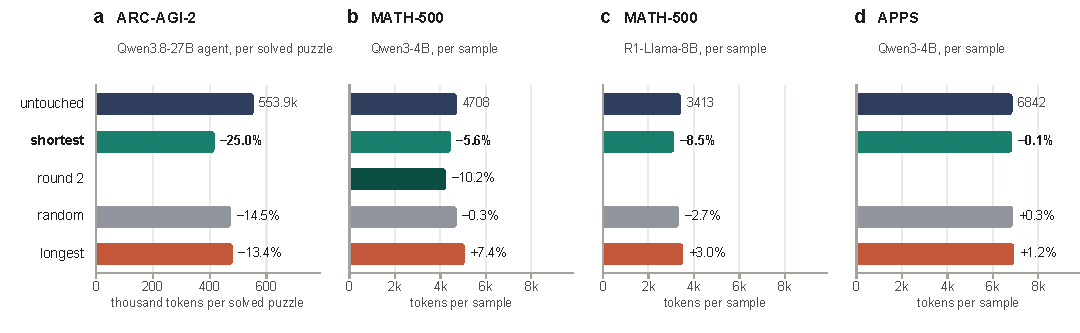
\includegraphics[width=\textwidth]{figS2.pdf}
\caption{\textbf{Token cost of every arm at the 8k cap (24k tokens per message for the ARC-AGI-2 agent).} Tokens per solved puzzle for the ARC-AGI-2 agent (thousands; all tokens of all seeds over all solves) and generated tokens per sample on MATH-500 and APPS (mean over seeds); labels give the change from the untouched model. At this cap shortest replay is the cheapest of the three replay rules in every setting and changes the cost relative to the untouched model by $-25.0\%$ (ARC-AGI-2), $-5.6\%$ (MATH-500, Qwen3-4B), $-8.5\%$ (MATH-500, R1-Llama-8B) and $-0.1\%$ (APPS).}
\label{fig:s2}
\end{figure}


\clearpage
\section*{Supplementary References}
\renewcommand{\refname}{}
\bibliography{../refs}
\end{document}
